\documentclass{article}

\usepackage[utf8]{inputenc}
\usepackage[T1]{fontenc}
\usepackage[spanish]{babel}
\usepackage{times}

\usepackage{color}
\definecolor{gray97}{gray}{.97}
\definecolor{gray75}{gray}{.75}
\definecolor{gray45}{gray}{.45}

\usepackage{listings}
\lstset{ frame=Ltb,
  framerule=0pt,
  aboveskip=0.5cm,
  framextopmargin=3pt,
  framexbottommargin=3pt,
  framexleftmargin=0.4cm,
  framesep=0pt,
  rulesep=.4pt,
  backgroundcolor=\color{gray97},
  rulesepcolor=\color{black},
%
  stringstyle=\ttfamily,
  showstringspaces = false,
  basicstyle=\small\ttfamily,
  commentstyle=\color{gray45},
  keywordstyle=\bfseries,
%
  numbers=left,
  numbersep=15pt,
  numberstyle=\tiny,
  numberfirstline = false,
  breaklines=true,
}

% minimizar fragmentado de listados
\lstnewenvironment{listing}[1][]
{\lstset{#1}\pagebreak[0]}{\pagebreak[0]}

\lstdefinestyle{consola}
{basicstyle=\scriptsize\bf\ttfamily,
  backgroundcolor=\color{gray75},
}

\lstdefinestyle{C}
{language=Python,
}

\usepackage{arxiv}

\usepackage[utf8]{inputenc} % allow utf-8 input
\usepackage[T1]{fontenc}    % use 8-bit T1 fonts
\usepackage{hyperref}       % hyperlinks
\usepackage{url}            % simple URL typesetting
\usepackage{booktabs}       % professional-quality tables
\usepackage{amsfonts}       % blackboard math symbols
\usepackage{nicefrac}       % compact symbols for 1/2, etc.
\usepackage{microtype}      % microtypography
\usepackage{lipsum}
\usepackage{graphicx}
\usepackage{import}
\usepackage{float}
\graphicspath{ {./images/} }

\usepackage{subcaption}

\setcounter{secnumdepth}{4}

\titleformat{\paragraph}

\title{TP 2.2 - GENERADORES DE NÚMEROS PSEUDOALEATORIOS DE DISTINTAS DISTRIBUCIONES DE PROBABILIDAD}


\author{
    Abud Santiago Elias \\
    Legajo 47015 \\
    \texttt{ sabudvicco@gmail.com} \\
    %% examples of more authors
    \And
    Buchhamer Ariel \\
    Legajo 46217\\
    \texttt{arielbuchhamer1@outlook.com} \\
    \And
    Castellano Marcelo \\
    Legajo 39028 \\
    \texttt{marce.geek22@gmail.com} \\
    \And
    Navarro Franco \\
    Legajo 46387 \\
    \texttt{franconavarro1889@gmail.com} \\
%% \AND
%% Coauthor \\
%% Affiliation \\
%% Address \\
%% \texttt{email} \\
%% \And
%% Coauthor \\
%% Affiliation \\
%% Address \\
%% \texttt{email} \\
%% \And
%% Coauthor \\
%% Affiliation \\
%% Address \\
%% \texttt{email} \\
}

\usepackage[spanish]{babel}
\usepackage{amsmath}
\begin{document}
  \maketitle
  \begin{abstract}
    El siguiente documento tiene por objetivo realizar un estudio sobre distintas distribuciones de probabilidad con sus respectivas características. De cada una se desarrollarán sus conceptos, se utilizará la tecnología para mostrar su funcionamiento y finalmente testear la generación de valores de las mismas.\end{abstract}

    \keywords{
    Simulación \and Números Pseudoaleatorios \and Distribución \and Probabilidad \and Discretas \and Continuas
    }



% keywords can be removed
%\keywords{First keyword \and Second keyword \and More}

  \section{Introducción}
  \label{sec:introducción}
  Se busca poder observar la generación de los distintos tipos de distribuciones a través de la generación
    de números pseudoaleatorios. Los tipos de distribuciones a desarrollar y analizar son tanto continuas como discretas, por lo que usaremos generadores específicos de cada uno.
    Luego de realizar las simulaciones, se procederá a aplicar el test de bondad Chi-Cuadrado a algunos de ellos para conocer su resultado.


  \section{Números Pseudoaleatorios}
  \label{sec:headings}
  Un número pseudoaleatorio no es más que el valor de una variable aleatoria x que tiene una distribución de probabilidad uniforme definida en el intervalo (0, 1).

  Los números pseudoaleatorios constituyen una parte realmente importante en la simulación de procesos estocásticos y generalmente se usan para generar el comportamiento de variables aleatorias, tanto continuas como discretas. Debido a que no es posible generar números realmente aleatorios, los consideramos como pseudoaleatorios, generados por medio de algoritmos determinísticos que requieren parámetros de arranque.

  Podemos asegurar con altos niveles de confiabilidad que el conjunto de números que utilizaremos en una simulación se comportan de manera muy similar a un conjunto de números totalmente aleatorios; por ello es que se les denomina números pseudoaleatorios.
  \section{Distribuciones de Probabilidad}

    En teoría de la probabilidad y estadística, la distribución de probabilidad de una variable
    aleatoria es una función que asigna a cada suceso definido sobre la variable aleatoria, la
    probabilidad de que dicho suceso ocurra. La distribución de probabilidad está definida
    sobre el conjunto de todos el rango de valores de la variable aleatoria.

    La distribución de probabilidad está completamente especificada por la función de distribución, cuyo valor en cada x
    real es la probabilidad de que la variable aleatoria sea menor o igual que x.
    Los tipos de variables existentes son:
    \item \textbf{Variable aleatoria:} Es aquella cuyo valor es el resultado de un evento aleatorio. Lo que quiere decir que son
    los resultados que se presentan al azar en cualquier evento o experimento.
    \item \textbf{Variable aleatoria discreta:} Es aquella que solo toma ciertos valores (frecuentemente enteros) y que resulta
  principalmente del conteo realizado.
    \item \textbf{Variable aleatoria continua:} Es aquella que resulta generalmente de la medición y puede tomar cualquier valor
    dentro de un intervalo dado

  A continuación se desarrollarán distintos generadores de valores de variables aleatorias a partir de las distribuciones probabilidad, las cuales están clasificadas según el tipo de variable.

  \subsection{Distribuciones Continuas de Probabilidad}
    \subsubsection{Distribución Uniforme}
  Se caracteriza por ser constante, en un intervalo entre a y b sin contener al cero. Surge del estudio de las características de los errores por redondeo al registrar un conjunto de medidas sujetas a cierto nivel de precisión.
  Sobresale respecto a las técnicas de simulación por su simplicidad y por el hecho de que se puede emplear para simular variables aleatorias a partir de case cualquier tipo de distribución de probabilidad.

  La función de densidad de probabilidad de la distribución uniforme continua es:
  \begin{equation}
    f{x} = \left\{\begin{array}{lcc}
                  \frac{1}{b-a} &   a<x<b \\
                  \\0, &no&esta&en&(a, b)
                  \end{array}
    \right.
  \end{equation}

  En esta ecuación  X es una variable aleatoria definida en (a, b)
  El valor esperado y la varianza de una variable aleatoria uniformemente distribuida, se puede representar por:
  \begin{equation}
    EX = \frac{b+a}{2}
  \end{equation}
  \begin{equation}
    VX = \frac{(b-a)^2}{12}
  \end{equation}

      \paragraph{Método de la transformación inversa para la distribución de probabilidad Uniforme}
  Para simular una distribución uniforme sobre cierto intervalo conocido (a,b) deberemos, en primer lugar, obtener la
  transformación inversa para la distribución uniforme acumulativa:

  \begin{equation}
    F(x) = \int_{0}^{a}\frac{1}{b-a}dt = \frac{x-a}{b-a} \ \text{  } \ 0 \leq F(x) \leq 1.
  \end{equation}

  Lo cual podemos deducir como su función inversa a:
  \begin{equation}
  x = a +(b-a)r \ \text{  }\ 0 \leq r \leq 1.
  \end{equation}

  En seguida, generamos un conjunto de números aleatorios correspondientes al rango de las probabilidades acumulativas,
  es decir, los valores de variables aleatorias uniformes definidas sobre el rango 0 a 1. Cada número aleatorio r determina,
  de manera única, un valor de la variable x uniformemente distribuida.

  \paragraph{Código en Python}
  \begin{lstlisting}[style = Python]
    def uniforme(a, b, rep: int = 1):
      x = []
      for i in range(rep):
          x.append(a + (b - a) * (round(random(), 4)))
      return x

  \end{lstlisting}

  En el código se puede observar el ingreso de dos valores a y b que expresan los limites de la distribución uniforme.
  Además cuenta con un parámetro 'rep' con el que cuentan este y los demás códigos de las distribuciones que permite ingresar la cantidad de repeticiones que se requieran.
  En todos los casos se generarán mil valores, y cada uno se generara a través del método de la transformación inversa
  con una variable r cuyo valor es generado por el generador Mersenne Twister propio de Python

  \paragraph{Análisis}


  \paragraph{Test}


  \subsubsection{Distribución Exponencial}

  En caso de que la ocurrencia de un evento en un intervalo corto, y si la ocurrencia de tal evento es, estadísticamente independiente respecto a la ocurrencia de otros eventos, entonces el intervalo de tiempo entre ocurrencias de eventos de este tipo estará distribuido en forma exponencial.
  Se dice que una variable aleatoria X tiene una distribución exponencial, si se puede definir a su función de densidad como:


  \begin{equation}
    f(x) = ae^{-ax}
  \end{equation}
  con a > 0 y x >= 0.
  La función de distribución acumulativa de X está dada por:
  \begin{equation}
    F(x) = \int_{0}^{a} ae^{-at}dt = 1-e^{-ax},
  \end{equation}
  y la media junto con la variancia de X se pueden expresar como
  \begin{equation}
    EX = \int_{0}^{\infty} xae^{-ax}dx = \frac{1}{a}
  \end{equation}
  \begin{equation}
    VX = \int_{0}^{\infty} (x-\frac{1}{a})^2 = \frac{1}{a^2} = (EX)^2
  \end{equation}

  \paragraph{Método de la transformación inversa para la distribución de probabilidad Exponencial}

  Existen muchas maneras para lograr la generación de valores de variables aleatorias exponenciales. Puesto que la
  distribución acumulativa existe explícitamente (vista en la ecuación (8)),la técnica de la transformación inversa nos permite desarrollar métodos directos para dicha generación.
  Debido a la simetría que existe entre la distribución uniforme sigue que la intercambiabilidad de F(x) y 1 - F(x). Por lo tanto:
  \begin{equation}
    r = e^{-ax}
  \end{equation}
  y consecuentemente
  \begin{equation}
    x = -\frac{1}{a}log r  = - EXlog r
  \end{equation}
  Por consiguiente, para cada valor del número pseudoaleatorio r, se determina un único valor para x. Los valores de
  x toman tan sólo magnitudes no negativas, debido a que el log (r) es ≤ 0 para ser 0 ≤ r ≤ 1 y además se ajustan a la
  función de densidad exponencial con un valor esperado x. Es importante notar que pese a que esta técnica parece en
  principio muy simple, es preciso recordar que en una computadora digital el cálculo logarítmico natural involucra una
  expansión en serie de potencias para cada valor de la variable aleatoria un informe que se debe generar.

  \paragraph{Código en Python}
  \begin{lstlisting}[style = Python]
    def exponencial(ex, rep: int = 1):
      x = []
      for i in range(rep):
          x.append(-ex * math.log(round(random(), 4)))
      return x

  \end{lstlisting}
  En el caso de la generación de valores para la distribución exponencial se generaran los valores a partir del método de la transformada inversa. El parámetro ex es la media de la distribución exponencial y
  la variable r cuyo valor es generado por el generador Mersenne Twister propio de Python.

  \paragraph{Análisis}

  \paragraph{Test}

  \subsubsection{Distribucion Gamma}
  Si un determinado proceso consiste de k eventos sucesivos y si el total del tiempo transcurrido para dicho proceso se puede considerar igual a la suma de k valores independientes de la variable aleatoria con distribución
  exponencial, cada uno de los cuales tiene un parámetro definido a la distribución de esta suma coincidirá con una distribución gamma con parámetros a y k.
  La función gamma está descrita mediante la siguiente función de densidad:
  \begin{equation}
    f(x) = \frac{a^{k}x^{(k-1)}e^{-ax}}{(k-1)!}
  \end{equation}
  donde a > 0, k > 9 y x se considera no negativo.
  Respecto a la media y la variancia de esta distribución, sus corrspondientes expresiones están formuladas como sigue:
  \begin{equation}
    EX = \frac{k}{a}
  \end{equation}
  \begin{equation}
    VX = \frac{k}{a^{x}}
  \end{equation}

  \paragraph{Código en Python}
  \begin{lstlisting}[style = Python]
   def gamma(k, a, rep: int = 1):
      x = []
      for i in range(1, rep):
          tr = 1
          for j in range(1, k):
              tr *= random()
          x.append(-(math.log(tr)) / a)
      return x
  \end{lstlisting}
  Para la distribución Gamma, se realizarán 1000 tiradas y se generaran los valores a partir del método de la transformada
  inversa. El parámetro k representa la cantidad de eventos sucesivos y a representa el parámetro lambda a utilizar.El valor
  de la variable r es generado por el generador Mersenne Twister propio de python.

  \paragraph{Análisis}


  \subsubsection{Distribución Normal}
  La distribución normal basa su utilidad en el teorema del límite central. Este postula que, la distribución de probabilidad de la sima de N valores
  de variable aleatoria x independientes pero idénticamente distribuidos, con medias respectivas u y variancias σ se aproximan asintóticamente a una distribución normal, a medida
  que N se hace muy grande.

  En consecuencia, el teorema del límite central permite el empleo de distribuciones normales para representar medidas globales operadas sobre los efectos de causas (errores)
  aditivas distribuidas en forma independiente sin importar la distribución de probabilidad a que obedezcan las mediciones de causas individuales.

  Si la variable aleatoria X tiene una función de densidad f(x) dada como:

  \begin{equation}
    f(x) = \frac{1}{σ_{x}\sqrt {2\pi}}e^{\frac{-(x-\mu)^2}{2σ^2}}
  \end{equation}

  El valor esperado y la variancia de la distribución normal están dados por:
  \begin{equation}
    EX = \mu_{x}
  \end{equation}
  \begin{equation}
    EX = \sigma_{x}^2
  \end{equation}

  \paragraph{Método de la transformación inversa para la distribución de probabilidad Normal}
  El procedimiento para simular valores normales utilizando computadoras requiere el uso de la suma de K valores de
  variables aleatorias distribuidos uniformemente; esto es la suma de r1, r2... rk con cada ri definida en el intervalo 0 <ri
  <1. Aplicando la convención notacional de la forma matemática del teorema central del límite, encontramos que:
  \begin{equation}
    \theta = \frac{a+b}{2} = \frac{0+1}{2} = \frac{1}{2},
  \end{equation}
  \begin{equation}
    \sigma = \frac{b-a}{\sqrt {12}} = \frac{1}{\sqrt {12}},
  \end{equation}
  \begin{equation}
    z = \frac{\sum_{i=2}^{K}r_{i}-K/2}{\sqrt {K/12}}
  \end{equation}
  Pero por definición, z es un valor de variable aleatoria con distribución normal estándar.
  Por lo tanto:

  \begin{equation}
    x = \sigma_{x}(\frac{12}{K})^{1/2}(\sum_{i=1}^{K}r_{i}-\frac{K}{2}) + \mu_{x}
  \end{equation}
  Por lo tanto, con la ecuación anterior, podemos proporcionar una formulación muy simple para generar valores de
  variable aleatoria normalmente distribuidos. Para generar un solo valor x bastará con sumar K números aleatorios
  definidos en el intervalo de 0 a 1. Este procedimiento se puede repetir tantas veces como valores de variables aleatorias
  normalmente distribuidos se quieran

  \paragraph{Código en Python}
  \begin{lstlisting}[style = Python]
    def normal(ex, stdx, rep: int = 1):
      x = []
      for i in range(rep):
          sm = 0
          for j in range(12):
              sm += random()
          x.append(stdx * (sm - 6) + ex)
      return x
  \end{lstlisting}
  En el código se puede observar como se ingresa como parámetro la media(ex) y la desviación estándar (stdx).Se
  generaran una cantidad arbitraria de valores a través del método de la transformación inversa con una variable r cuyo
  valor es generado por Python.

  \paragraph{Análisis}

  \paragraph{Test}

  \subsection{Distribuciones Discretas de Probabilidad}
  \subsubsection{Distribución Pascal}
  Cuando los procesos de ensayos de Bernoulli se repiten hasta lograr que ocurran k éxitos (k > 1), la variable aleatoria que caracteriza al número de fallas tendrá una distribución binomial negativa.
  Por consiguiente, los valores de variables aleatorias con distribución binomial negativa coinciden esencialmente con la suma de k valores de variable aleatoria con distribución geométrica; en este caso, k es un
  número entero y la distribución recibe el nombre de distribución de Pascal.

  La función de distribución de probabilidad para una distribución binomial negativa está dada por:

  \begin{equation}
    f(x) = (\frac{k+x-1}{x})p^{k}q^{x} \ \text{   } \ x = 0,1,2,...,
  \end{equation}
  donde k es el número total de éxitos en una sucesión de k + x ensayos, con x el número de fallas que ocurren antes de obtener k éxitos.

  El valor esperado y la variancia de X se representa con:

  \begin{equation}
    EX = \frac{kq}{p}
  \end{equation}
  \begin{equation}
    VX = \frac{kq}{p^2}
  \end{equation}

  \paragraph{Código en Python}
  \begin{lstlisting}[style = Python]
    def pascal(k, q, rep: int = 1):
      nx = []
      for i in range(rep):
          tr = 1
          for j in range(k):
              tr *= random()
          x = math.log(tr) // math.log(q)
          nx.append(x)
      return nx
  \end{lstlisting}

  \subsubsection{Distribución Binomial}
  La distribución binomial proporciona la probabilidad de que un evento o acontecimiento tenga lugar x veces en un conjunto de n ensayos,
  donde la probabilidad de éxito está dada por p. La función de probabilidad para la distribución binomial se puede expresar de la manera siguiente:

  \begin{equation}
    f(x) = \binom{n}{x} p^{x}q^{n-x}
  \end{equation}
  donde x se toma como un entero definido en el intervalo finito 0,1,2,...n, y al que se le asocio el valor q = (1-p).

  El valor esperado y la variancia de la variable binomial X son
  \begin{equation}
    EX = np
  \end{equation}

  \begin{equation}
  VX = npq
  \end{equation}

  \paragraph{Código en Python}
  \begin{lstlisting}[style = Python]
   def binomial(n, p, rep: int = 1):
      x = []
      for i in range(rep):
          y = 0
          for j in range(1, n):
              if (random() - p) < 0:
                  y += 1
          x.append(y)
      return x
  \end{lstlisting}

  \paragraph{Test}

  \subsubsection{Distribución Hipergeométrica}

  \section{Gráficas}
  \subsection{Con capital infinito}
  \subsubsection{Estrategia martingala}
  \begin{figure}[H]
    \centering
    \begin{subfigure}{0.5\textwidth}
      \centering
      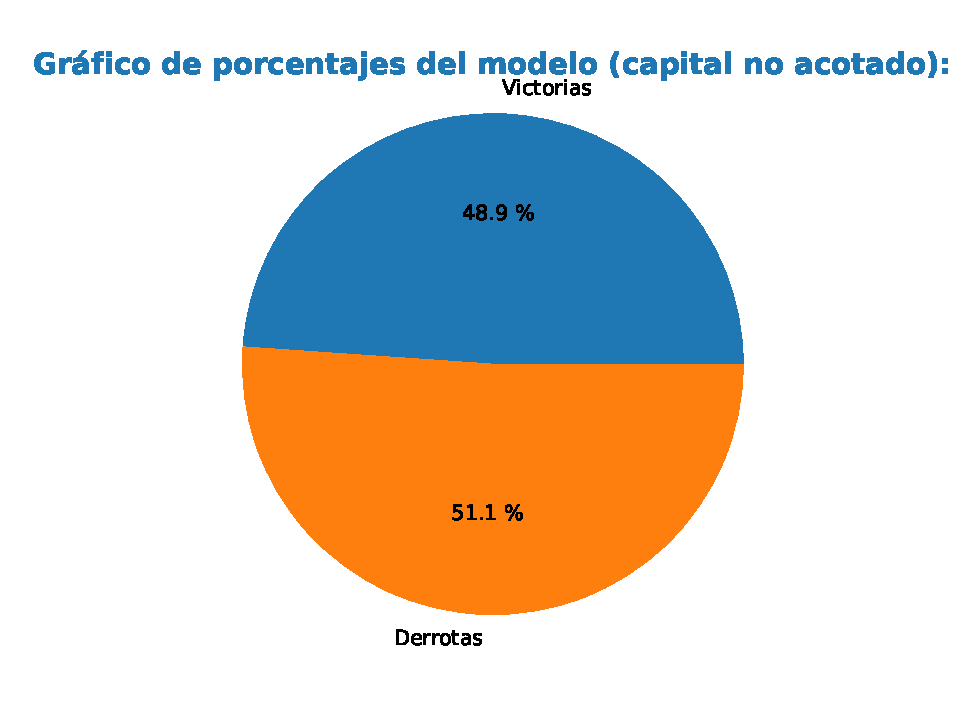
\includegraphics[width=0.8\textwidth]{generated/porcentajes-martingala-no acotado.pdf}
      \caption{Porcentajes de victorias vs. derrotas}
    \end{subfigure}%
	\begin{subfigure}{0.5\textwidth}
	  \centering
      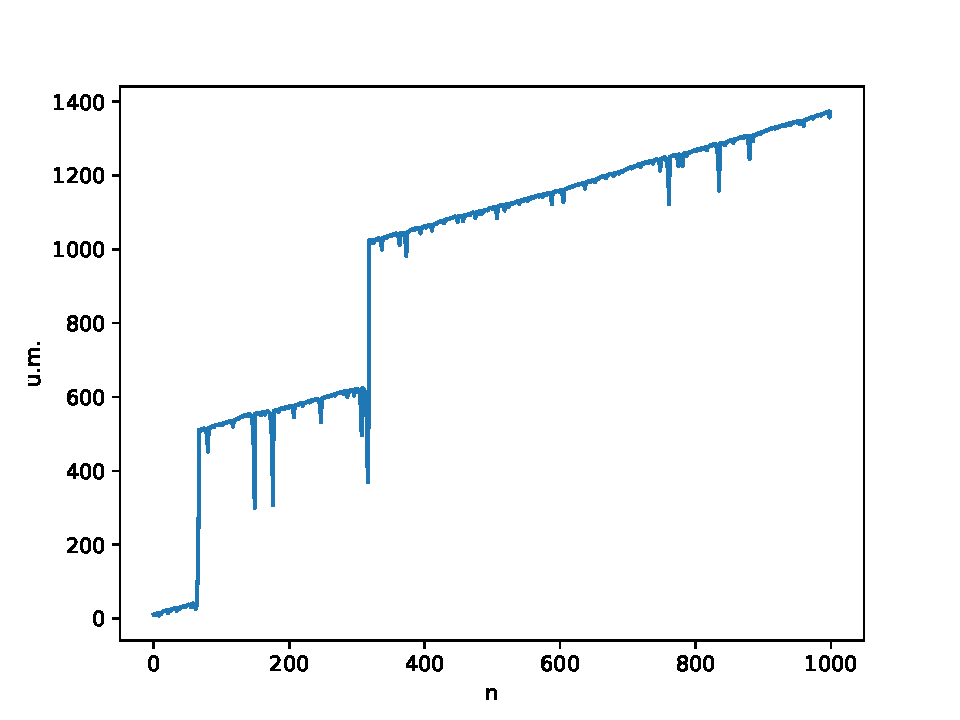
\includegraphics[width=0.8\textwidth]{generated/capital-martingala-no acotado.pdf}
	  \caption{Flujo de caja}
	\end{subfigure}
	\caption{resultados obtenidos aplicando la estrategia martingala en 25 corridas de $n = 1000$ rondas (con capital infinito)}
  \end{figure}

  \subsubsection{Estrategia d’Alembert}
  \begin{figure}[H]
    \centering
    \begin{subfigure}{0.5\textwidth}
      \centering
      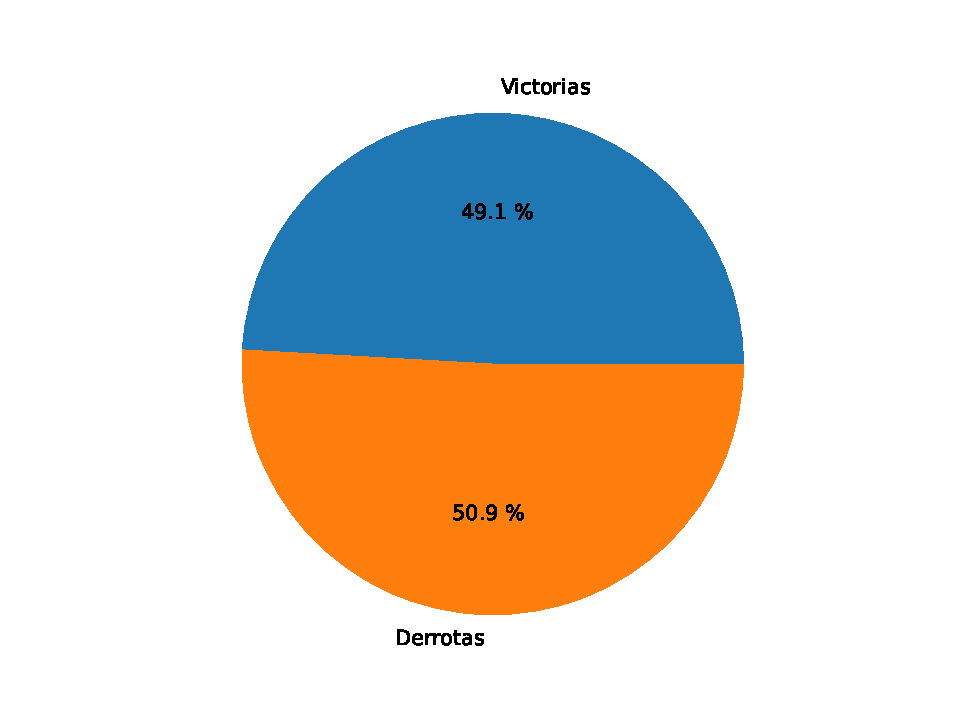
\includegraphics[width=0.8\textwidth]{generated/porcentajes-d'alembert-no acotado.pdf}
      \caption{Porcentajes de victorias vs. derrotas}
    \end{subfigure}%
    \begin{subfigure}{0.5\textwidth}
      \centering
      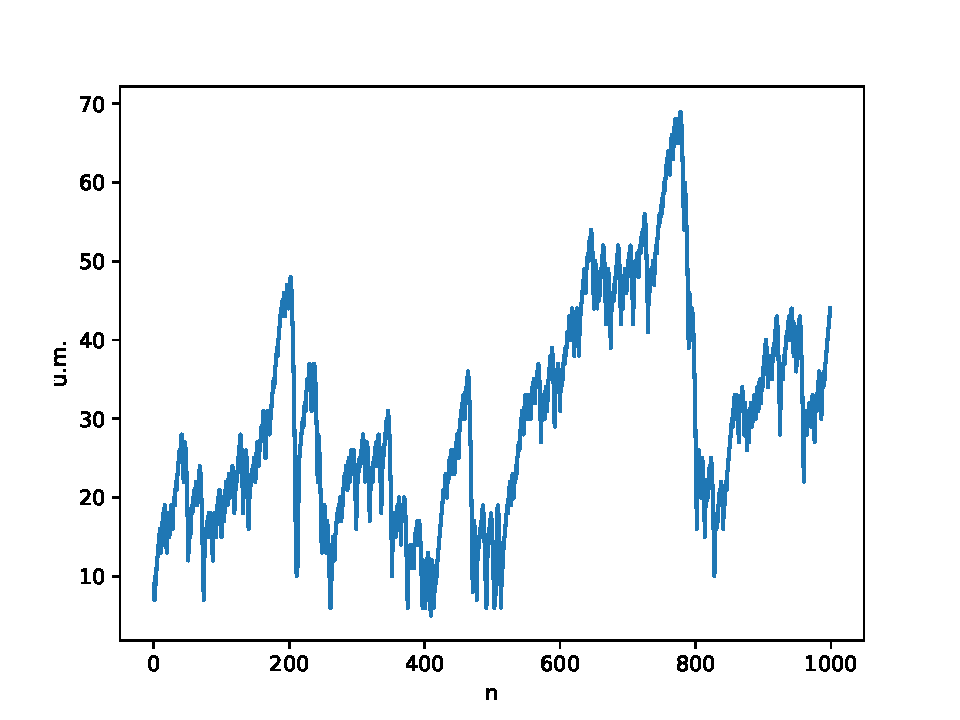
\includegraphics[width=0.8\textwidth]{generated/capital-d'alembert-no acotado.pdf}
      \caption{Flujo de caja}
    \end{subfigure}
    \caption{resultados obtenidos aplicando la estrategia d’Alembert en 25 corridas de $n = 1000$ rondas (con capital infinito)}
  \end{figure}

  \subsubsection{Estrategia Fibonacci}
  \begin{figure}[H]
    \centering
    \begin{subfigure}{0.5\textwidth}
      \centering
      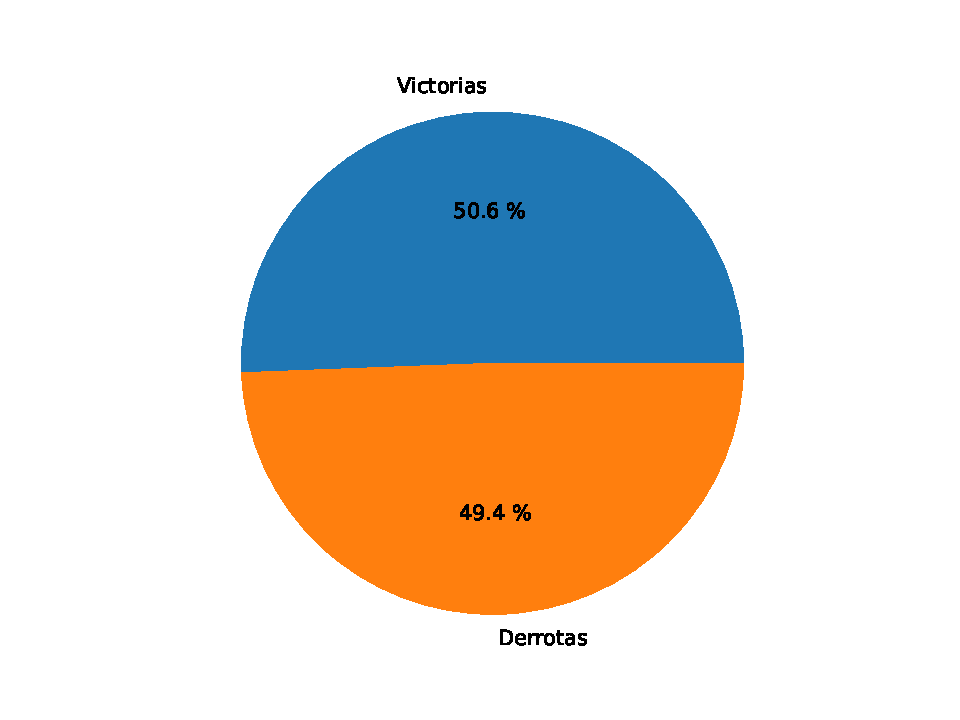
\includegraphics[width=0.8\textwidth]{generated/porcentajes-fibonacci-no acotado.pdf}
      \caption{Porcentajes de victorias vs. derrotas}
    \end{subfigure}%
    \begin{subfigure}{0.5\textwidth}
      \centering
      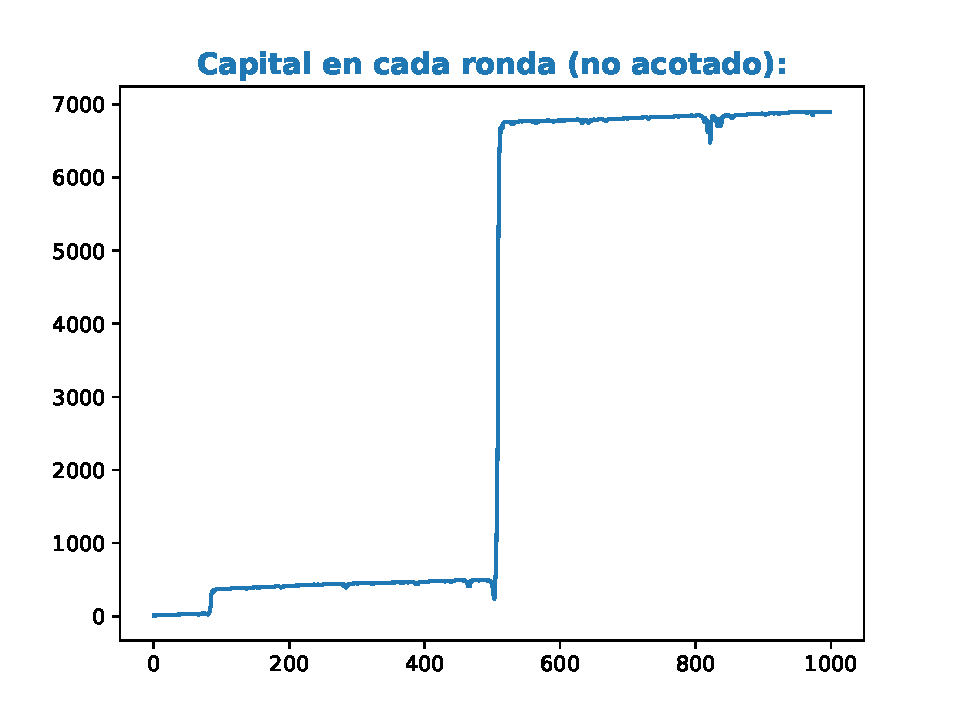
\includegraphics[width=0.8\textwidth]{generated/capital-fibonacci-no acotado.pdf}
      \caption{Flujo de caja}
    \end{subfigure}
    \caption{resultados obtenidos aplicando la estrategia Fibonacci en 25 corridas de $n = 1000$ rondas (con capital infinito)}
  \end{figure}

  \subsubsection{Resumen}

  Vemos que las diferentes estrategias logran resultados muy beneficiosos, pero muy raramente y luego de perder todo el
  capital reiteradas veces.

  \subsection{Con capital acotado}
  \subsubsection{Estrategia martingala}
  \begin{figure}[H]
    \centering
    \begin{subfigure}{0.5\textwidth}
      \centering
      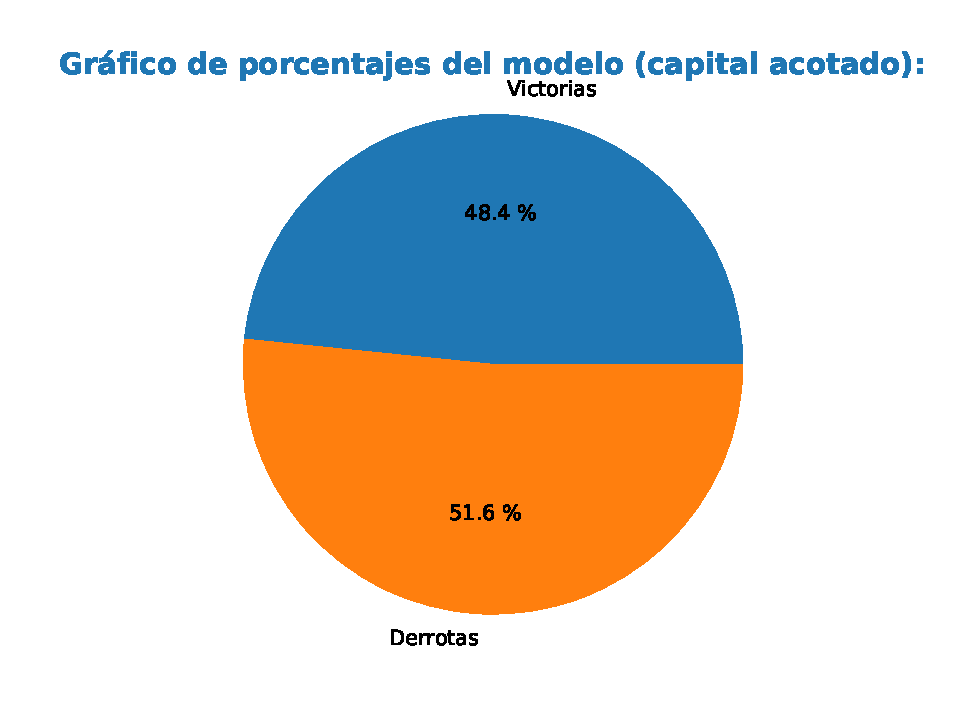
\includegraphics[width=0.8\textwidth]{generated/porcentajes-martingala-acotado.pdf}
      \caption{Porcentajes de victorias vs. derrotas}
    \end{subfigure}%
	\begin{subfigure}{0.5\textwidth}
	  \centering
	    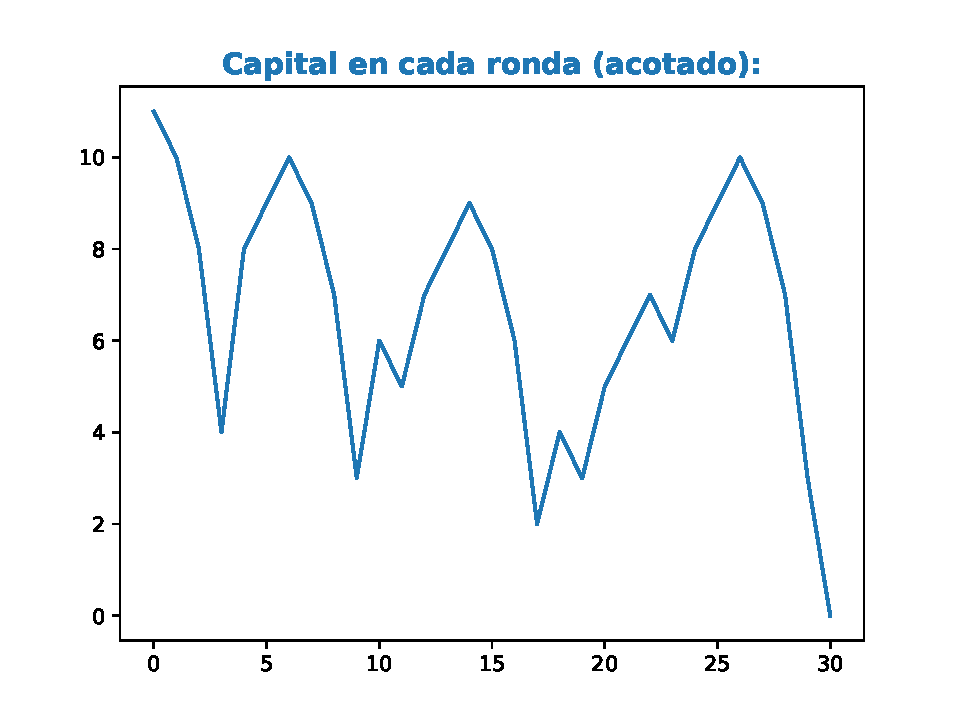
\includegraphics[width=0.8\textwidth]{generated/capital-martingala-acotado.pdf}
      \caption{Flujo de caja}
    \end{subfigure}
    \caption{resultados obtenidos aplicando la estrategia martingala en 25 corridas (con capital acotado)}
  \end{figure}

  \subsubsection{Estrategia d’Alembert}
  \begin{figure}[H]
    \centering
    \begin{subfigure}{0.5\textwidth}
      \centering
      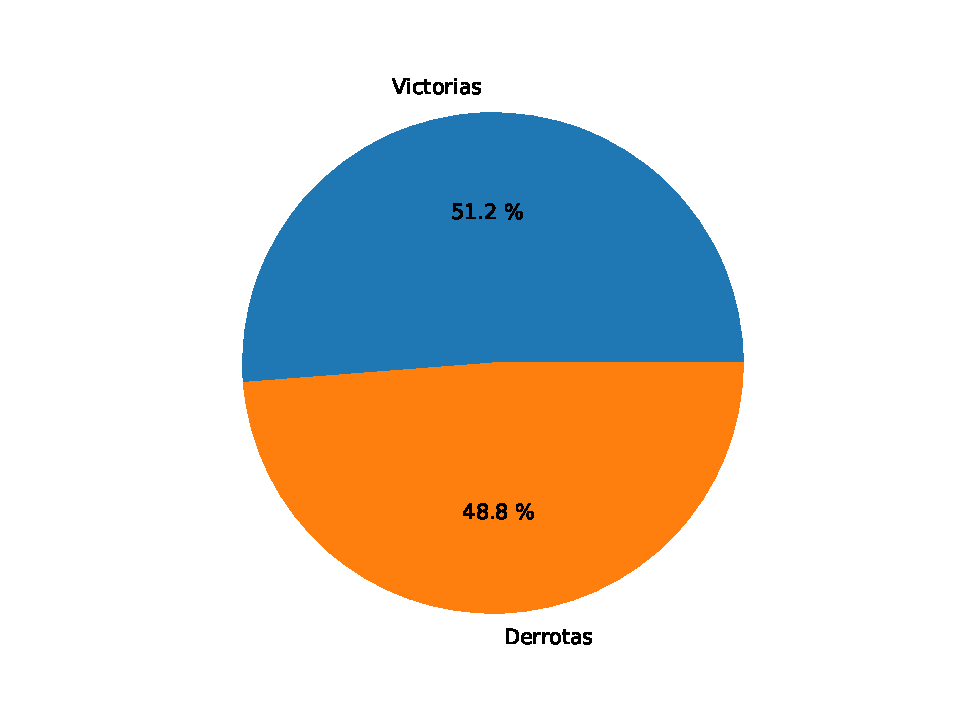
\includegraphics[width=0.8\textwidth]{generated/porcentajes-d'alembert-acotado.pdf}
      \caption{Porcentajes de victorias vs. derrotas}
    \end{subfigure}%
    \begin{subfigure}{0.5\textwidth}
      \centering
      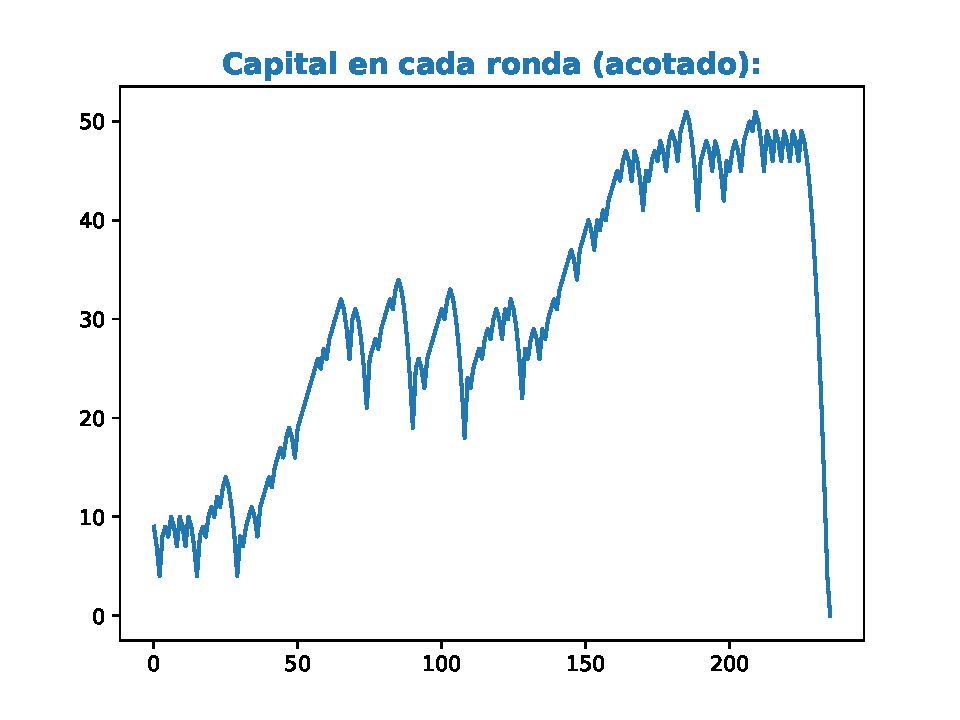
\includegraphics[width=0.8\textwidth]{generated/capital-d'alembert-acotado.pdf}
      \caption{Flujo de caja}
    \end{subfigure}
    \caption{resultados obtenidos aplicando la estrategia d’Alembert en 25 corridas (con capital acotado)}
  \end{figure}

  \subsubsection{Estrategia Fibonacci}
  \begin{figure}[H]
    \centering
    \begin{subfigure}{0.5\textwidth}
      \centering
      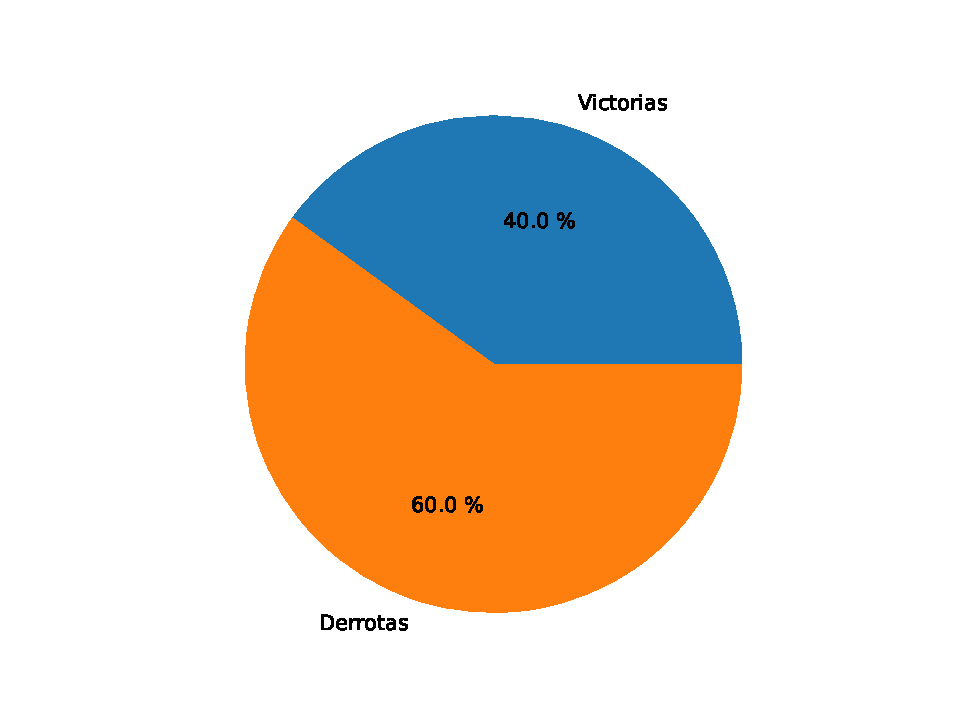
\includegraphics[width=0.8\textwidth]{generated/porcentajes-fibonacci-acotado.pdf}
    \end{subfigure}%
    \begin{subfigure}{0.5\textwidth}
      \centering
      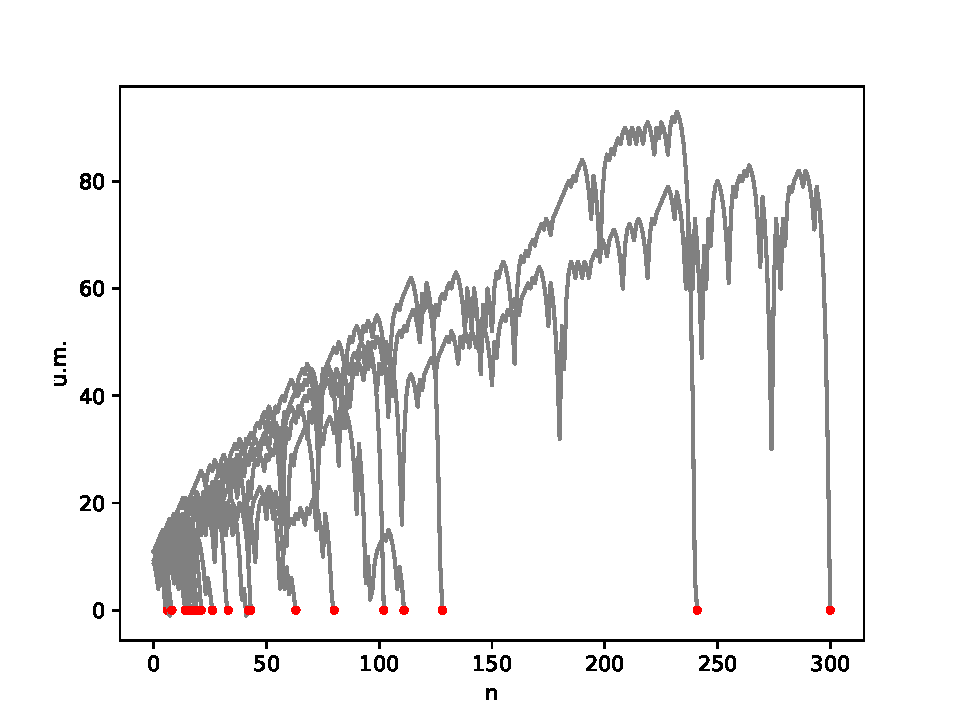
\includegraphics[width=0.8\textwidth]{generated/capital-fibonacci-acotado.pdf}
    \end{subfigure}
    \caption{resultados obtenidos aplicando la estrategia Fibonacci en 25 corridas (con capital acotado)}
  \end{figure}

  \subsubsection{Resumen}

  Si bien en algunos casos se ha llegado a mantener un capital creciente por más de 200 rondas y se han obtenido
  ganancias de más de 60 veces el capital inicial, la verdad es que la mayoría de las rondas no se han extendido a más
  de 40 rondas, y las ganancias de estos casos no han subido a más de 30 veces la apuesta inicial.

  \subsection{Resumen general de las tiradas}
  \begin{figure}[H]
    \centering
    \begin{subfigure}{0.5\textwidth}
      \centering
      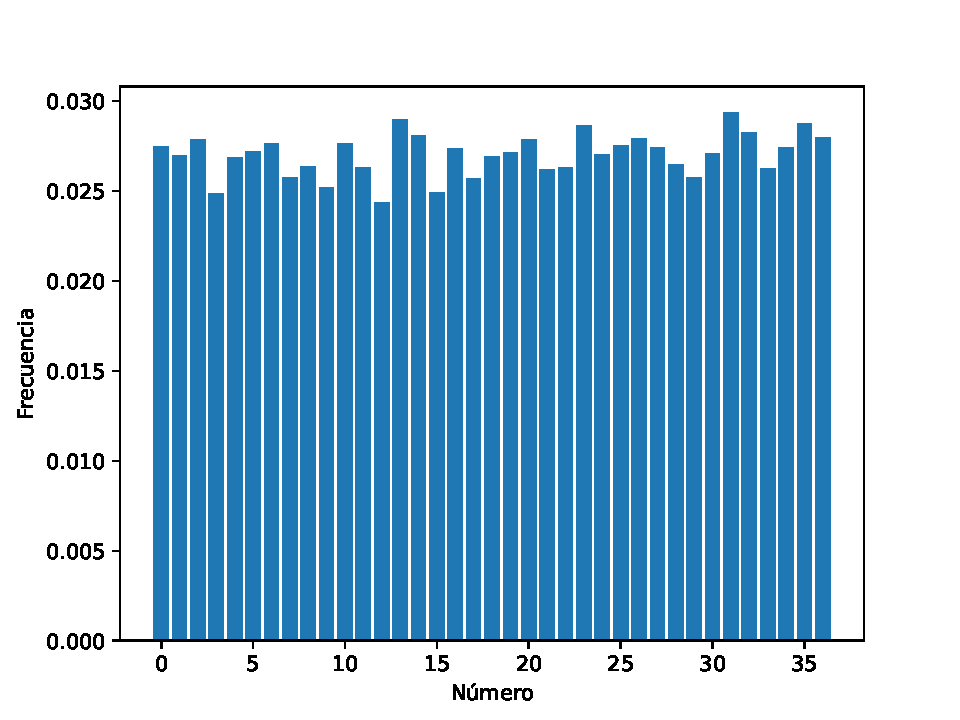
\includegraphics[width=0.8\textwidth]{generated/frec-aparicion.pdf}
      \caption{Frecuencias relativas de aparición por cada número}
    \end{subfigure}%
    \begin{subfigure}{0.5\textwidth}
      \centering
      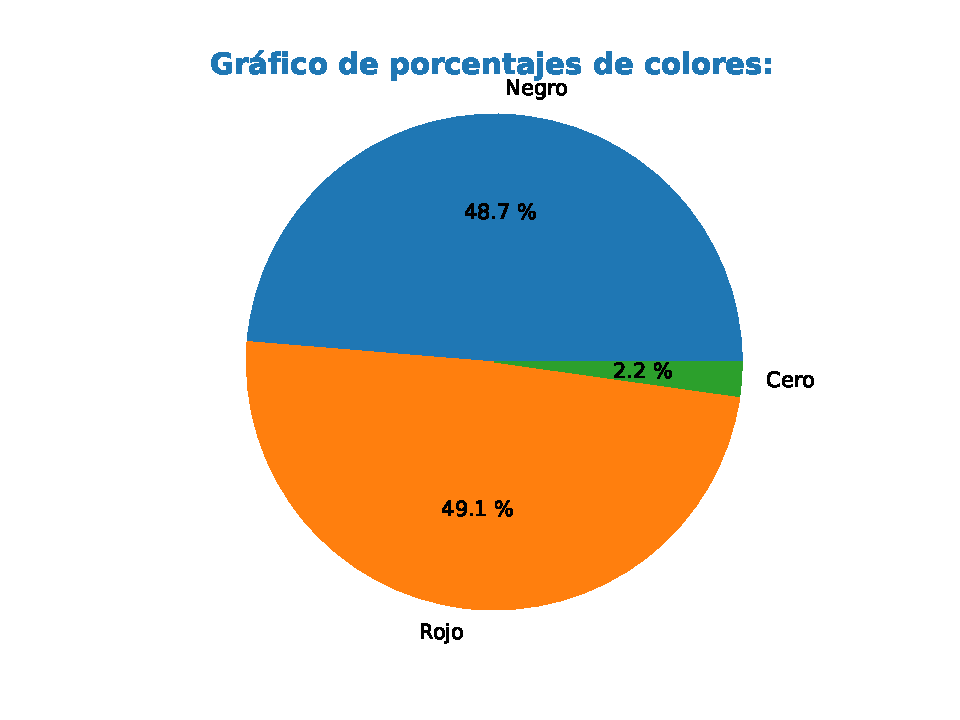
\includegraphics[width=0.8\textwidth]{generated/resumen-colores.pdf}
      \caption{Porcentajes de colores}
    \end{subfigure}
  \end{figure}

\section{Conclusiones}

    Con lo obtenido y trabajado hasta el momento, queda demostrado que estas estrategias no ofrecen resultados
    consistentes y su desempeño es tan azaroso como el juego al que están sujetas.

    Otra observación que se puede hacer es que, aunque no son buenas estrategias a largo plazo, sí ofrecen una gran
    posibilidad de obtener pocas ganancias en un corto plazo, evidenciado por la gran cantidad de veces que las
    estrategias, aún con capital acotado, han sobrevivido y obtenido ganancias tras unas pocas rondas.


\section{Referencias}
  \label{sec:referencias}
    https://astridmll.wordpress.com/2016/09/13/numeros-pseudoaleatorios-y-sus-caracteristicas/
    https://ansenuza.unc.edu.ar/comunidades/bitstream/handle/11086.1/1346/DistribC3%B3n%20de%20Probabilidades%20Discretas.pdf?sequence=1&isAllowed=y
\end{document}
